\chapter{Tích phân Monte Carlo }\label{ch:2}
\section{Tổng quát}\label{sec:2.1}
Giá trị kỳ vọng của một hàm biến ngẫu nhiên $f(\textbf{x})$. 
\begin{align}
	\textbf{E}[f(\textbf{x})]=\int{f(\textbf{x})P(\textbf{x})d\textbf{x}} 
\end{align}
với $P(\textbf{x})$ là  là phân phối xác suất của biến ngẫu nhiên $\textbf{x}$\\
Phương sai của biến ngẫu nhiên $\textbf{x}$.
\begin{align}
	Var(\textbf{x})=\textbf{E}[(\textbf{x}-\textbf{E}[X])^2]=\textbf{E}[\textbf{x}^2]-\textbf{E}[\textbf{x}]^2
\end{align}
Xét tích phân Monte Carlo cơ bản, với hàm tích phân một chiều $f(x)$ từ a đến b.
\begin{align}
	\textbf{F}=\int{f(x)dx}
\end{align}
Như hình $ \ref{tichphan} $ tích phân của hàm $f(x)$ có giá trị là diện tích bên dưới đường cong của hàm. 
Giả sử chọn một điểm ngẫu nhiên $x$ nằm trong đoạn $[a, b]$, tính hàm $f(x)$ tại x và quả với $(b-a)$. Hình $ \ref{tichphan} $ cho thấy kết quả là một hình chữ nhật, trong đó $f(x)$ là chiều cao và $(b-a)$ chiều rộng của nó.
\begin{figure}[H]
	\centering
	\begin{subfigure}{5cm}
		\centering
		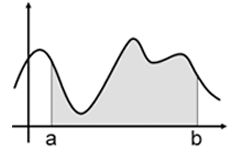
\includegraphics[width=0.9\textwidth]{2_1.png}
		\label{Sneutrino tadpole}
	\end{subfigure}
	\begin{subfigure}{5cm}
		\centering
		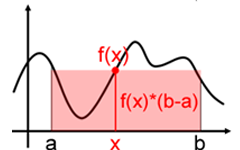
\includegraphics[width=1\textwidth]{2_2.png}
		\label{Sneutrino tadpole}
	\end{subfigure}
	\caption{Tích phân trên miền [a,b] là diện tích dưới đường cong.}\label{tichphan}
   \end{figure}
   \begin{figure}[H]
	\centering
	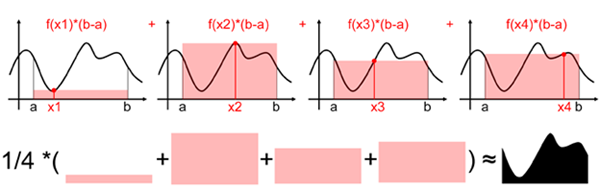
\includegraphics[width=0.9\textwidth]{2_3.png}
	\caption{Giá trị tích phân gần được khi chọn các điểm ngẫu nhiên x}\label{tichphan1}
   \end{figure}
   Nếu tính giá trị hàm tại $x1$, kết quả tính toán sẽ khá thấp, tính giá trị hàm tại $x2$ thì kết quả diện tích khá lớn. 
   Nhưng khi tiếp tục tính toán hàm tại các điểm ngẫu nhiên khác nhau giữa a và b, 
   cộng diện tích của các hình chữ nhật và tính trung bình, kết quả sẽ gần đúng với kết quả chính xác của tích phân.
   Và cách tính trung bình các hình chữ nhật này sẽ hội tụ đến diện tích của hàm tích phân khi số lượng mẫu được sử dụng trong phép tính tăng lên. 
   Như minh họa minh họa trong hình $ \ref{tichphan1} $. Giả sử tính tích phân tại bốn điểm ngẫu nhiên. 
   Lấy kết quả của hàm f(x) tại 4 điểm ngẫu nhiên của x nhân với (b-a) và tính trung bình. 
   Như vậy kết quả sẽ được xấp xỉ với kết quả chính xác.
\section{Tích phân Monte Carlo với hàm mật độ xác suất đều}\label{sec:2.2}
Giá trị trung bính của $\langle{F^N}\rangle$ khi biến ngẫu nhiên $X_i$ là phân bố đều
\begin{align}
	\langle{F^N}\rangle=(b-a)\frac{1}{N}\sum_{i=0}^{N-1}{f(x_i)}
\end{align}
Trong đó $N$ là số lượng mẫu, $X_i$ là biến ngẫu nhiên phân bố đều trong khoảng $[a,b]$. Và xác suất của mỗi Xi đều bằng $\frac{1}{b-a}$
Theo định luật số lớn thì số mẫu N càng tăng đến vô cùng thì phép tính tích phân Monte Carlo sẽ hội tụ đến kết quả chính xác.
\begin{align}
	P(lim_{N\rightarrow\infty}{\langle{F^N}\rangle}=F)=1
\end{align}
$\langle{F^N}\rangle$ là một biến ngẫu nhiên, với $pdf(x_i)=\frac{1}{b-a}$. Giá trị kỳ vọng được tính như sau:
\begin{equation} 
	\begin{split}
		{E}[\langle{F^N}\rangle] & = {E}\left[{(b-a)\frac{1}{N}\sum_{i=0}^{N-1}{f(X_i)}}\right]\\
										 & = (b-a)\frac{1}{N}{E}[f(x)]\\
										 & = (b-a)\frac{1}{N}\sum_{i=0}^{N-1}\int_a^b{f(x)pdf(x)dx}\\
										 & = \frac{1}{N}\sum_{i=0}^{N-1}\int_a^b{f(x)dx}\\
										 & = \int_a^b{f(x)dx}\\
										 & = F
	\end{split}
\end{equation}	
\section{Tích phân Monte Carlo với hàm mật độ xác suất bất kỳ}\label{sec:2.3}
Để mở rộng tích phân Monte Carlo với hàm phân bố bất kỳ. Trong đó với $pdf(X_i)$ là hàm mật độ xác suất của biến ngẫu nhiên $X_i$  thì $\langle{F^N}\rangle$ được xác định như sau.
\begin{align}
	\langle{F^N}\rangle=frac{1}{N}\sum_{i=0}^{N-1}{\frac{f(X_i)}{pdf(X_i)}}
\end{align}
Giá trị kỳ vọng được tính như sau:
\begin{equation} 
	\begin{split}
		{E}[\langle{F^N}\rangle] & = {E}\left[{\frac{1}{N}\sum_{i=0}^{N-1}\frac{{f(X_i)}}{pdf(X_i)}}\right] \\
										 & = \frac{1}{N}\sum_{i=0}^{N-1}{E}\left[\frac{{f(X_i)}}{pdf(X_i)}\right]\\
										 & = \frac{1}{N}\sum_{i=0}^{N-1}\int_\Omega{\frac{{f(X_i)}}{pdf(X_i)}}{pdf(x)dx}\\
										 & = \frac{1}{N}\sum_{i=0}^{N-1}\int_\Omega{f(x)dx}\\
										 & = \int_\Omega{f(x)dx}\\
										 & = \int_a^b{f(x)dx}\\
										 & = F
\end{split}
\end{equation}
\section{Giảm phương sai}\label{sec:2.4}
Giảm phương sai thì kết quả tích phân sẽ trở nên chính xác hơn. Do không phụ thuộc vào số lượng mẫu như đã đề cập tại phương trình $ \ref{ct1.17} $ thì phương sai của $\langle{F^N}\rangle$ như sau.
\begin{equation} 
	\begin{split}
		{\sigma}^2{\left[\langle{F^N}\rangle\right]}&={\sigma}^2\left[{\frac{1}{N}\sum_{i=0}^{N-1}\frac{{f(X_i)}}{pdf(X_i)}}\right] \\
										 & = \frac{1}{N^2}\sum_{i=0}^{N-1}{\sigma}^2\left[{\frac{{f(X_i)}}{pdf(X_i)}}\right]\\
										 & = \frac{1}{N^2}\sum_{i=0}^{N-1}{\sigma}^2\left[Y_i\right]\\
										 & = \frac{1}{N}{\sigma}^2\left[Y\right]
	\end{split}
\end{equation}
Và độ lệch chuẩn với $Y_i=\frac{f(X_i)}{pdf(X_i)}$ 
\begin{equation}
	\left[\langle{F^N}\rangle\right]=\frac{1}{\sqrt{N}}\sigma[Y]\label{ct2.10}
\end{equation}
Phương trình $ \ref{ct2.10} $ đã chứng minh rằng lệch chuẩn hội tụ với $O(\sqrt{N})$. 
Phương trình này cũng cho thấy bằng cách giảm phương sai của mỗi $Y_i$, chúng ta có thể giảm phương sai của ${\sigma}{\left[\langle{F^N}\rangle\right]}$
